\documentclass[a4paper, 14pt]{extarticle}
\usepackage{../generalPreamble}
\usepackage{../conspectFormat}
\usepackage{../nonFancyTOC}
\usepackage{../russianLocale}

\lhead{}

\title{Экзаменационные вопросы по ЦОС}
\author{Корытов Павел, 6304 \\ СПбГЭТУ \enquote{ЛЭТИ}}
\date{\today}
\begin{document}
\maketitle

\setcounter{secnumdepth}{4}
\setcounter{tocdepth}{1}
\tableofcontents{}
\section{Обобщенная схема ЦОС}
\begin{figure}[h]
    \centering
    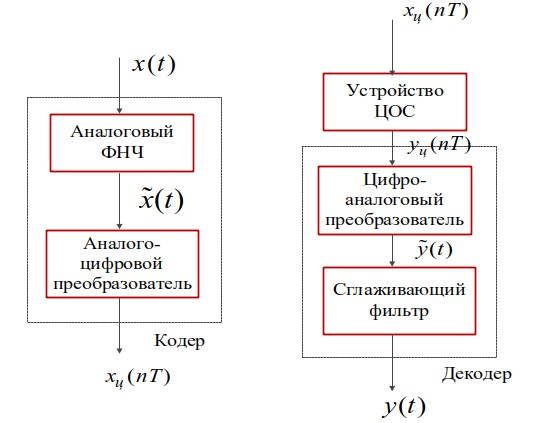
\includegraphics[width=0.4\textwidth]{img/S001.jpg}
\end{figure}
Исходная информация в обобщенной схеме ЦОС --- \textbf{аналоговый сигнал} ($x(t)$ или $s(t)$), т.е. непрерывная фукнкция времени.

\begin{enumerate}
    \item Аналоговый сигнал подается на вход аналогового \textbf{ФНЧ (фильтр нижних частот)}.

        ФНЧ синтезируется одним из известных методов и выполняет роль ограничителя спектра сигнала. Это необходимо для дальнейшего применения \textbf{теоремы Котельникова}.

        После пропускания через аналоговый ФНЧ меняется форма сигнала, сигнал становится \textbf{ограниченным по спектру}.
    \item Переход от аналогового сигнала к \textbf{дискретному} (применение \textbf{процедуры дискретизации})
        \begin{tcolorbox}[title=Теорема Котельникова]
            Любой сигнал с ограниченным спектром может быть без потерь информации представлен набором дискретных отсчётов, взятых через интервал $T$, удовлетворяющий условию:
            \begin{equation*}
                T \le \frac{1}{2f_\text{в}}; f_\text{д} \ge 2f_\text{в}, 
            \end{equation*}
            где:
            \begin{itemize}
                \item $T$ --- период дискретизации сигнала,
                \item $f_\text{в} $ --- верхняя граничная частота,
                \item $f_\text{д}$ --- частота дискретизации сигнала.
            \end{itemize}

            После дискретизации сигнал \textbf{дискретный} --- квантованный по времени, но аналоговый по уровню (состоянию). Отсчёты расположены через равноотстоящие промежутки --- \textbf{период дискретизации}

        \end{tcolorbox}
    \item Переход от дискретного сигнала к \textbf{цифровому}

        \textbf{Аналогово-цифровой преобразователь (АЦП)} преобразует значения из аналоговых в цифровые. Дискретизация и квантование выполняются с помощью ПО.

        \textbf{Квантование} сопровожается \textbf{ошибкой (шумом) квантования} 
    \item Обработка цифрового сигнала

        \textbf{Система ЦОС} --- выполняет преобразование сигнала в соответствии с решаемой задачей. На выходе сигнал \textbf{цифровой} --- квантованный по времени и по состоянию.


    \item Обратное преобразование от цифрового сигнала в аналоговый

        \textbf{Цифро-аналоговый преобразователь (ЦАП)} --- преобразует цифровой сигнал в ступенчатый аналоговый. Является ФНЧ с низкой степенью избирательности.
    \item Устранение ступенчатого эффекта.

        \textbf{Cглаживающий фильтр} --- ФНЧ, устраняющий ступенчатый эффект. 
\end{enumerate}

\section{Типовые последовательности ЦОС}
\subsection{Цифровой единичный импульс}
\begin{figure}[h]
    \centering
    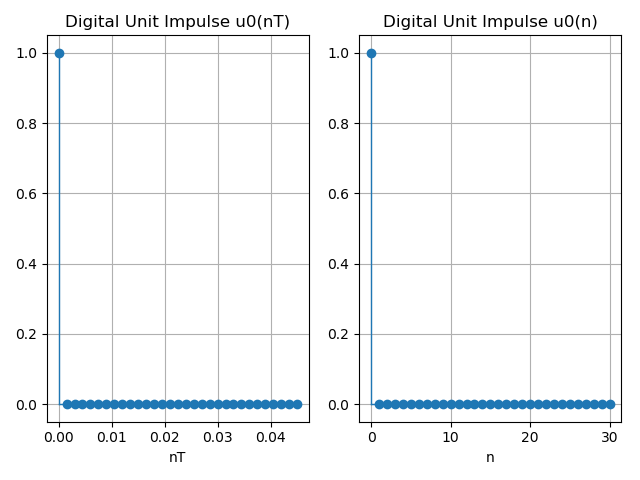
\includegraphics[width=0.7\textwidth]{img/signals/1.png}
    \caption{Цифровой единичный импульс}%
\end{figure}
\begin{equation}
    u_0 (nT) = \begin{cases}
        1, &n = 0;\\
        0, &n \ne 0.
    \end{cases}
\end{equation}

\clearpage
\subsection{Цифровой единичный скачок}
\begin{figure}[h]
    \centering
    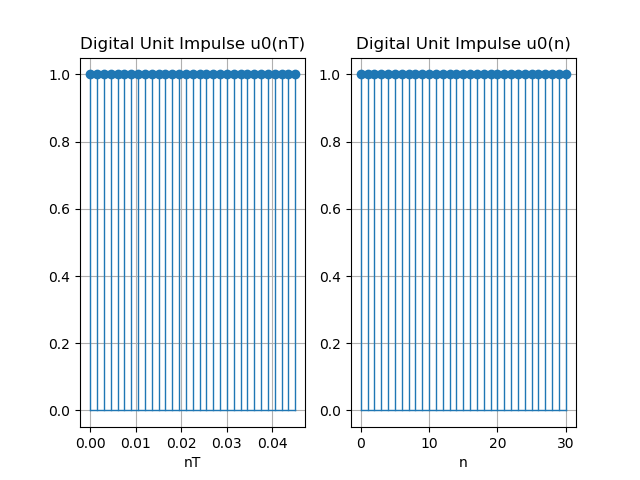
\includegraphics[width=0.7\textwidth]{img/signals/2.png}
    \caption{Цифровой единичный скачок}%
\end{figure}
\FloatBarrier{}
\textbf{Цифровой единичный скачок} --- результат дискретизации аналогового скачка.
\begin{equation}
    u_1 (nT) = \begin{cases}
        1, &n \ge 0;\\
        0, &n < 0.
    \end{cases}
\end{equation}

\clearpage
\subsection{Дискретная экспонента}
\begin{figure}[h]
    \centering
    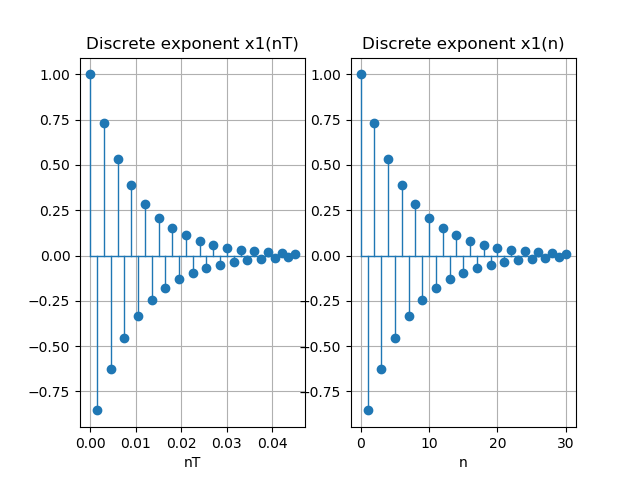
\includegraphics[width=0.7\textwidth]{img/signals/3.png}
    \caption{Дискретная экспонента}%
    \label{img:}
\end{figure}

\textbf{Дискретная экспонента} --- результат дискретизации аналоговой экспоненты.

\begin{equation}
    x_1(n) = \begin{cases}
        a^n, &n \ge 0 \\
        0, &n < 0,
    \end{cases}
\end{equation}
где $n$ --- дискретное нормированное время. От $a$ зависит, будет ли сменяться знак экспоненты.

\clearpage
\subsection{Дискретный гармонический сигнал}
\begin{equation}
    x_2(n) = C \cos (\hat{ \omega_0 } n),
\end{equation}
где $C$ --- амплитуда сигнала, $\hat{ \omega_0 }$ --- частота сигнала

\subsection{Дискретный комплексный гармонический сигнал}
\begin{figure}[h]
    \centering
    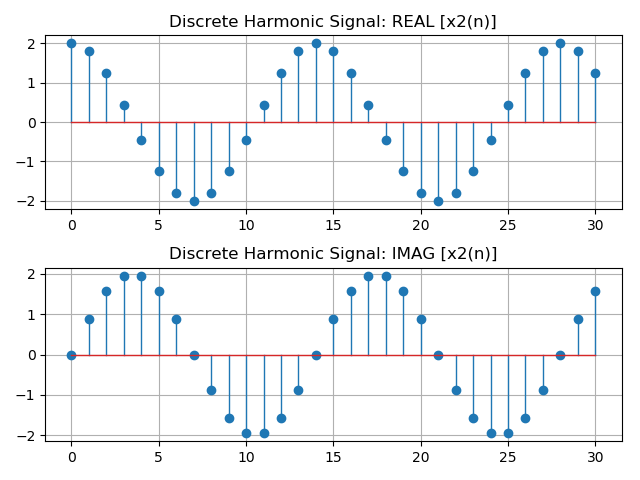
\includegraphics[width=0.7\textwidth]{img/signals/4.png}
    \caption{Графики вещественной и комплексной частей гармонического сигнала}%
\end{figure}

\begin{equation}
    x_2(n) = C e ^{j\hat{ \omega_0 } n}
\end{equation}

\clearpage
\subsection{Дискретный прямоугольный импульс}
\begin{figure}[h]
    \centering
    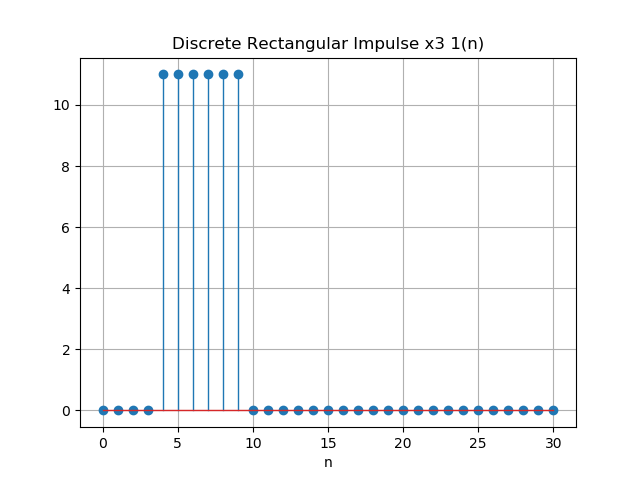
\includegraphics[width=0.7\textwidth]{img/signals/6.png}
    \caption{График дискретного прямоугольного импульса}%
\end{figure}
\begin{equation}
    x_3 (n) = \begin{cases}
        U, &n_0 \le n \le (n_0 + n_\text{imp} --- 1 );\\
        0, &\text{иначе},
    \end{cases}
\end{equation}
где $U$ --- амплитуда, $n_0$ --- момент начала, $n_\text{imp} $ --- длительность.

\clearpage
\subsection{Дискретный треугольный импульс}
\begin{figure}[h]
    \centering
    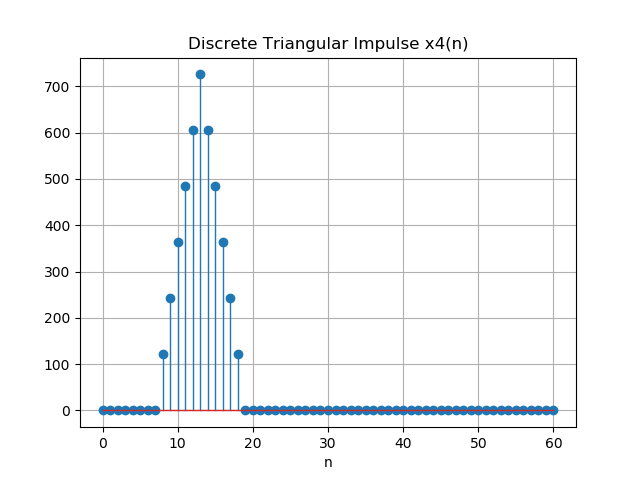
\includegraphics[width=0.7\textwidth]{img/signals/7.png}
    \caption{График дискретного треугольного импульса}
\end{figure}
Можно получить сверткой дискретного прямоугольного импульса самим с собой на интервале $L$.

Аналитическая запись свертки:
\begin{equation}
    x_4(t) = x_3(t) * x_3(t) = \sum\limits_{\tau = 0}^{N} x_3(\tau) x_3(t - \tau),
\end{equation}
где $x_3(\tau)$:
\begin{equation}
    x_3(\tau) = \begin{cases}
        U, & n_0 \le \tau \le (n_0 + n_{imp} - 1)\\
        0, & \text{иначе}
    \end{cases}
\end{equation}
Длина свертки: $L = 2N - 1$.


\section{Линейные дискретные системы. Описание во временной области}
\subsection{Линейные дискретные системы}\label{subsec:lds}
\textbf{Система обработки сигнала} --- объект, выполняющий требуемое преобразование входного сигнала \textbf{(воздействия)} в выходной \textbf{(реакцию)}.

\begin{figure}[h]
    \centering
    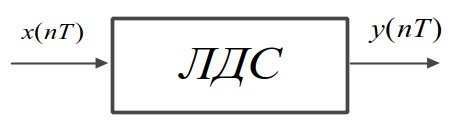
\includegraphics[width=0.6\textwidth]{img/S002.jpg}
    \caption{Схематичное изображение ЛДС}%
\end{figure}

Система --- \textbf{линейная}, если она отвечает условиям \textbf{аддитивности} и \textbf{однородности}.

\textbf{Аддитивность} --- реакция на сумму воздействий равна сумме реакций на воздействия:

\textbf{Однородность} --- воздействию, умноженному на весовой коэффициент, соответствует реакция, умноженная на тот коэффициент.

\begin{equation}
    L\{ a_1 x_1(n) \pm a_2 x_2(n) \pm \ldots \} = a_1 L\{ x_1(n)\} \pm a_2 L\{x_2(n)\} \pm \ldots,
\end{equation}
где: $x_i(n)$ --- воздействие, $a_i$ --- весовой коэффициент.

Система --- \textbf{дискретная}, если она преобразует дискретное воздействие в дискретную реакцию.

Система --- \textbf{стационарная}, если её реакция инвариантна по отношению к начала отсчёта времени. По умолчанию рассматриваем стационарные линейные дискретные системы (ЛДС).

% TODO НДУ?

\subsection{Описание ЛДС во временной области}
Основная характеристика во временной области --- \textbf{импульсная характеристика (ИХ)}, $h(n)$ --- реакция на цифровой единичный импульс $u_0(n)$ при ННУ.

\textbf{Соотношение вход/выход} ЛДС --- однозначно связано с ИХ, имеет вид линейной свертки:
\begin{equation}
    y(nT) = \sum^{\infty}_{m=0} h[ (n - m)T ] x(mT) = \sum^{\infty}_{m=0} h(mT) x [ (n-m)T ],
\end{equation}
\begin{equation}
    y(n) = \sum^{\infty}_{m=0} h(n-m)x(m) = \sum^{\infty}_{m=0} h(m) x(n-m).
\end{equation}

\textbf{Передаточная функция} --- однозначно связана с соотношением вход/выход, имеет вид \textbf{разностного уравнения (РУ)}:
\begin{equation}
    y(n) = \underbrace{\sum^{N-1}_{i=0} b_i x(n-i)}_\text{Нерекурсивная часть} - \underbrace{\sum^{M-1}_{k=1} a_k y(n-k)}_\text{Рекурсивная часть}, 
\end{equation}
где:
\begin{itemize}
    \item $b_i, a_k$ --- вещественные константы (параметры ЛДС)
    \item $i, k$ --- задержки воздействия, реакции
    \item $(N-1), (M-1)$ --- константы (максимальные задержки)
    \item $x(n)$ --- воздействие
    \item $y(n)$ --- реакция
\end{itemize}

Вычисление реакции по формуле свертки или разностому уравнению осуществляется методов приямой подстановке при начальных нулевых условиях.

Типы ЛДС:
\begin{itemize}
    \item \textbf{Рекурсивные} --- реакция зависит от текущего и предшествующих отсчётов воздействия и предшествующих отсчётов реакции.
        
        $ \exists k: a_k \ne 0$.

        Имеют бесконечную ИХ \textbf{(БИХ-ЛДС)}.
    \item \textbf{Нерекурсивные} --- реакция зависит только от текущего и предшествующих отсчётов воздействия и не зависит от отсчётов реакции.

        $\forall k: a_k = 0$.

        Имеют конечную ИХ \textbf{(КИХ-ЛДС)}. ИХ КИХ-ЛДС совпадает с коэффициентами $b_i$: $h(n) = b_i, n=i$
\end{itemize}

\section{Линейные дискретные системы. Описание в $z$-области}
См.~\ref{subsec:lds} (\nameref{subsec:lds}).

Основная характеристика --- \textbf{передаточная функция} (ПФ) --- $z$-изображение импульской характеристики:
\begin{equation}
    H(z) = \sum^{N-1}_{n=0} h(n) z^{-n} = \frac{Y(z)}{X(z)},
\end{equation}
где $Y(z)$ --- $z$-изображение реакции, $X(z)$ --- $z$-изображение воздействия.

Передаточная функция с использованим разностного уравнения:
\begin{equation}
    H(z) = \frac{ \sum^{N-1}_{i=0} b_i z^{-i} }{1 + \sum^{M-1}_{k=1} a_k z^{-k}},
\end{equation}
где:
\begin{itemize}
    \item $z^{-i}, z^{-k}$ --- задержки воздействия и реакции,
    \item $a_k$ --- коэффициенты передаточной функции.
\end{itemize}

Для нерекурсивных ЛДС:
\begin{equation}
    H(z) = \sum^{N-1}_{i=0} b_i z^{-i} = \sum^{N-1}_{n=0} h(n) z^{-n}.
\end{equation}

\textbf{Порядок рекурсивной ЛДС} равен порядку знаменателя передаточной функции $(M-1)$ при условии $(N-1) \le (M-1)$.

\textbf{Порядок нерекурсивной ДЛС} равен $(N-1)$.

\textbf{Нули ПФ} --- корни числителя, \textbf{Полюса (особые точки) ПФ} --- корни знамененателя. \textbf{Карта нулей и полюсов} --- $z$-плоскость с единичной окружностью, нулями и полюсами.

Нули и полюсы --- попарно комплексно сопряженные числа.

Для \textbf{устойчивой ЛДС} полюса расположены внутри единичной окружности.

ПФ рекурсивных ЛДС может быть представлена следующими разновидностями:
\begin{itemize}
    \item Произведение простейших множителей:
        \begin{equation}
            H(z) = b_0 \prod^{M-1}_{k=1} \frac{1 - z_{0^k}z^{-1}}{1-z_{*^k}z^{-1}},
        \end{equation}
        где:
        \begin{itemize}
            \item $z_{0^k}$ --- $k$-й нуль, $z_{*^k}$ --- $k$-й полюс.
        \end{itemize}
    \item Произведение множителей второго порядка:
        \begin{equation}
            H(z) = \prod^{L}_{k=1} \frac{b_{0k} + \tilde{b}_{1k} z^{-1} + \tilde{b}_{2k}z^{-2}}{1 + a_{1k} z^{-1} + a_{2k} z^{-2}},
        \end{equation}
        где:
        \begin{itemize}
            \item $b_{0k}, \tilde{b}_{1k}, \tilde{b}_{2k}, a_{1k}, a_{2k}$ --- вещественные коэффициенты рекурсивных звеньев 2-го порядка (биквадратов),
            \item $L$ --- количество звеньев:
                \begin{equation}
                L = int( \frac{M-1}{2} ).
                \end{equation}
        \end{itemize}
    \item Сумма простых дробей:
        \begin{equation}
            H(z) = \sum^{M-1}_{k=1} H_k(z) = \sum^{M-1}_{k=1} \frac{A_k}{1-z_{*^k}z^{-1}}, 
        \end{equation}
        где:
        \begin{itemize}
            \item $z_{*^k}$ --- простой (некратный) полюс,
            \item $A_k$ --- коэффициент разложения при полюсе.
        \end{itemize}
\end{itemize}

\section{Линейные дискретные системы. Описание в частотной области}
См.~\ref{subsec:lds} (\nameref{subsec:lds}).
Основная характеристика --- \textbf{комплексная частотная характеристика} --- Фурье-изображение ИХ:
\begin{equation}
    H(e^{j \hat{ \omega }}) = \sum^{\infty}_{n=0} h(n) e^{-j \hat{ \omega } n},
\end{equation}
где $\hat{ \omega }$ --- нормированная частота (рад):
\begin{equation}
    \hat{ \omega } = \omega T.
\end{equation}

Связь ЧХ и ПФ:
\begin{equation}
    H(e^{j \hat{ \omega }}) = H(z) \big\vert_{z=e^{j \hat{w}}} = \dfrac{ \sum\limits^{N-1}_{i=0} b_i e^{-ji \hat{ \omega }} }{1 + \sum\limits^{M-1}_{k=1} a_k e^{-jk \hat{ \omega }}},
\end{equation}
где:
\begin{itemize}
    \item $b_i$ --- параметры нерекурсивной части ЛДС,
    \item $a_i$ --- параметры рекурсивной части ЛДС.
\end{itemize}

В показательной форме:
\begin{equation}
    H(e^{j \hat{ \omega }}) = \left| H(e^{j \hat{ \omega }}) \right| e^{j \cdot \arg \{ H(e^{j \hat{ \omega }}) \} } = A(\hat{ \omega }) e^{j \varphi(\hat{ \omega })},
\end{equation}
где $A(\hat{ \omega })$ --- АЧХ, $\varphi( \hat{ \omega } )$ --- ФЧХ.

\textbf{Амлитудно-частотная характеристика (АЧХ)} --- частотная зависимость отношения амплитуды реакции к амплитуде гармонического воздействия в установившемся режиме.

\textbf{Фазочастнотная характеристика (ФЧХ)} --- частотная зависимость разности фаз реакции и гармонического воздействия в установившемся режиме.

Свойства АЧХ и ФЧХ:
\begin{itemize}
    \item АЧХ и ФЧХ --- периодические функции;
    \item АЧХ --- четная функция частоты, ФЧХ --- нечетная;
    \item АЧХ и ФЧХ рассчитываются в основной полосе частот для систем с вещественными параметрами;
    \item по карте нулей и полюсов можно определить местоположение минимумов, максимумов и нулей АЧХ в основной полосе частот;
    \item Частота комплексно сопряженного полюса соответствует частоте максимума АЧХ (приблизительно);
    \item Частота комплексно сопряженного нуля соответствует частоте минимума АЧХ (приблизительно), если радиус-вектор полюса меньше 1, и нуля АЧХ, если радиус-вектор равен 1. В точке нуля АЧХ наблюдается скачок на $\pi$;
    \item Вещественным нулям соответствует нуль АЧХ на границе основной полосы частот $0$ и/или $\pi$.
\end{itemize}

\section{Основные характеристики ЛДС. Соотношение вход/выход. Устойчивость ЛДС}
\lipsum[1] %TODO

\section{$z$-преобразование и его свойства}
\lipsum[1] %TODO

\section{Структруы ЛДС}
\lipsum[1] %TODO

\section{Цифровые фильтры}
\lipsum[1] %TODO

\section{Синтех КИХ-фильтров методом окон}
\lipsum[1] %TODO

\section{Синтез КИХ-фильтров методом наилучшей равномерной (чебышевской) аппроксимации}
\lipsum[1] %TODO

\section{Синтез БИХ-фильтров}
\lipsum[1] %TODO

\section{Описание дискретных сигналов в $z$-области}
\lipsum[1] %TODO

\section{Описание дискретных сигналов в частотной области}
\lipsum[1] %TODO

\section{Дискретное преобразование Фурье (ДПФ)}
\lipsum[1] %TODO

\section{Методы непараметрического спектрального анализа}
\lipsum[1] %TODO

\section{Методы параметрического спектрального анализа}
\lipsum[1] %TODO

\section{Адаптивные фильтры и их применения}
\lipsum[1] %TODO


\end{document}
